% Options for packages loaded elsewhere
\PassOptionsToPackage{unicode}{hyperref}
\PassOptionsToPackage{hyphens}{url}
%
\documentclass[
  ignorenonframetext,
  aspectratio=169,
]{beamer}
\usepackage{pgfpages}
\setbeamertemplate{caption}[numbered]
\setbeamertemplate{caption label separator}{: }
\setbeamercolor{caption name}{fg=normal text.fg}
\beamertemplatenavigationsymbolsempty
% Prevent slide breaks in the middle of a paragraph
\widowpenalties 1 10000
\raggedbottom
\setbeamertemplate{part page}{
  \centering
  \begin{beamercolorbox}[sep=16pt,center]{part title}
    \usebeamerfont{part title}\insertpart\par
  \end{beamercolorbox}
}
\setbeamertemplate{section page}{
  \centering
  \begin{beamercolorbox}[sep=12pt,center]{part title}
    \usebeamerfont{section title}\insertsection\par
  \end{beamercolorbox}
}
\setbeamertemplate{subsection page}{
  \centering
  \begin{beamercolorbox}[sep=8pt,center]{part title}
    \usebeamerfont{subsection title}\insertsubsection\par
  \end{beamercolorbox}
}
\AtBeginPart{
  \frame{\partpage}
}
\AtBeginSection{
  \ifbibliography
  \else
    \frame{\sectionpage}
  \fi
}
\AtBeginSubsection{
  \frame{\subsectionpage}
}
\usepackage{amsmath,amssymb}
\usepackage{iftex}
\ifPDFTeX
  \usepackage[T1]{fontenc}
  \usepackage[utf8]{inputenc}
  \usepackage{textcomp} % provide euro and other symbols
\else % if luatex or xetex
  \usepackage{unicode-math} % this also loads fontspec
  \defaultfontfeatures{Scale=MatchLowercase}
  \defaultfontfeatures[\rmfamily]{Ligatures=TeX,Scale=1}
\fi
\usepackage{lmodern}
\ifPDFTeX\else
  % xetex/luatex font selection
\fi
% Use upquote if available, for straight quotes in verbatim environments
\IfFileExists{upquote.sty}{\usepackage{upquote}}{}
\IfFileExists{microtype.sty}{% use microtype if available
  \usepackage[]{microtype}
  \UseMicrotypeSet[protrusion]{basicmath} % disable protrusion for tt fonts
}{}
\makeatletter
\@ifundefined{KOMAClassName}{% if non-KOMA class
  \IfFileExists{parskip.sty}{%
    \usepackage{parskip}
  }{% else
    \setlength{\parindent}{0pt}
    \setlength{\parskip}{6pt plus 2pt minus 1pt}}
}{% if KOMA class
  \KOMAoptions{parskip=half}}
\makeatother
\usepackage{xcolor}
\newif\ifbibliography
\usepackage{graphicx}
\makeatletter
\def\maxwidth{\ifdim\Gin@nat@width>\linewidth\linewidth\else\Gin@nat@width\fi}
\def\maxheight{\ifdim\Gin@nat@height>\textheight\textheight\else\Gin@nat@height\fi}
\makeatother
% Scale images if necessary, so that they will not overflow the page
% margins by default, and it is still possible to overwrite the defaults
% using explicit options in \includegraphics[width, height, ...]{}
\setkeys{Gin}{width=\maxwidth,height=\maxheight,keepaspectratio}
% Set default figure placement to htbp
\makeatletter
\def\fps@figure{htbp}
\makeatother
\setlength{\emergencystretch}{3em} % prevent overfull lines
\providecommand{\tightlist}{%
  \setlength{\itemsep}{0pt}\setlength{\parskip}{0pt}}
\setcounter{secnumdepth}{-\maxdimen} % remove section numbering
\ifLuaTeX
\usepackage[bidi=basic]{babel}
\else
\usepackage[bidi=default]{babel}
\fi
\babelprovide[main,import]{english}
% get rid of language-specific shorthands (see #6817):
\let\LanguageShortHands\languageshorthands
\def\languageshorthands#1{}
\usepackage{pgfpages}
\usepackage{microtype}
\usepackage{tikz}
  \usetikzlibrary{positioning}
  \usetikzlibrary{arrows}
  \usetikzlibrary{graphs}

\definecolor{CTred}{RGB}{229,32,32}
\definecolor{CTgrey}{RGB}{153,153,153}

\usepackage{array}
\usepackage{dcolumn}
\newcolumntype{d}{D{.}{.}{-1}}
\usepackage{booktabs}
\usepackage{threeparttable}

% colors: white text on 90% black background
\setbeamercolor{normal text}{fg=black,bg=white}

% light blue as a highlight color
\setbeamercolor*{structure}{fg=CTred}
\setbeamercolor{section title}{fg=CTred}
\setbeamercolor{alerted text}{use=structure,fg=CTred}
\setbeamercolor*{palette primary}{use=structure,fg=structure.fg}
\setbeamercolor*{palette secondary}{use=structure,fg=structure.fg!95!black}
\setbeamercolor*{palette tertiary}{use=structure,fg=structure.fg!90!black}
\setbeamercolor*{palette quaternary}{use=structure,fg=structure.fg!95!black,bg=black!80}

\setbeamercolor*{framesubtitle}{fg=white}


% use system fonts: here, Gill Sans
\usefonttheme{professionalfonts}
\setbeamerfont{quote}{shape=\upshape}

% eliminate silly beamer navigation line at bottom of slides
\setbeamertemplate{navigation symbols}{}
\setbeamertemplate{footline}[frame number]

% ensure text jusfication
\usepackage{ragged2e}
\justifying

% pandoc makes 2nd-lever headers into blocks, and this ensures justification
% in blocks too
\addtobeamertemplate{block begin}{}{\justifying}




\urlstyle{same}
\usepackage[overlay,absolute]{textpos}

\setbeamertemplate{items}[square]

\TPGrid[10 mm,8 mm]{9}{8}
% beamer's left and right margin is 10 mm. The top/bottom margin is ??
% or without a header ??
% the slide dimensions are 128 mm x 96 mm
% so the resulting \TPHorizModule = 12 mm and \TPVertModule = 10 mm

% uncomment if you want biblatex for citations on slides

% \usepackage{csquotes}
% \usepackage[notes,short,noibid,backend=biber]{biblatex-chicago}
% \bibliography{course.bib} 

\providecommand{\exhibit}[2]{\includegraphics[keepaspectratio, height=0.9\textheight, width=\textwidth]{assets/img/#1}\\ {\tiny #2}}

\providecommand{\smallcite}[1]{({\footnotesize #1})}
\ifLuaTeX
  \usepackage{selnolig}  % disable illegal ligatures
\fi
\IfFileExists{bookmark.sty}{\usepackage{bookmark}}{\usepackage{hyperref}}
\IfFileExists{xurl.sty}{\usepackage{xurl}}{} % add URL line breaks if available
\urlstyle{same}
\hypersetup{
  pdftitle={Success and geography: Evidence from open-source software},
  pdfauthor={Gábor Békés (CEU, HUN-REN KRTK, and CEPR); Julian Hinz (Bielefeld University and Kiel Institute for the World Economy); Miklós Koren (CEU, HUN-REN KRTK, CEPR and CESifo); Aaron Lohmann (Bielefeld University and Kiel Institute for the World Economy)},
  pdflang={en},
  hidelinks,
  pdfcreator={LaTeX via pandoc}}

\title{Success and geography: Evidence from open-source software}
\author{Gábor Békés (CEU, HUN-REN KRTK, and CEPR) \and Julian Hinz
(Bielefeld University and Kiel Institute for the World
Economy) \and Miklós Koren (CEU, HUN-REN KRTK, CEPR and
CESifo) \and Aaron Lohmann (Bielefeld University and Kiel Institute for
the World Economy)}
\date{June 21, 2024\footnote<.->{This work was funded by the European
  Union under the Horizon Europe grant 101061123. Views and opinions
  expressed are, however, those of the author(s) only and do not
  necessarily reflect those of the European Union or the European
  Commission. Neither the European Union nor the granting authority can
  be held responsible for them.}}

\begin{document}
\frame{\titlepage}

\begin{frame}{Authors' dispersion in space}
\protect\hypertarget{authors-dispersion-in-space}{}
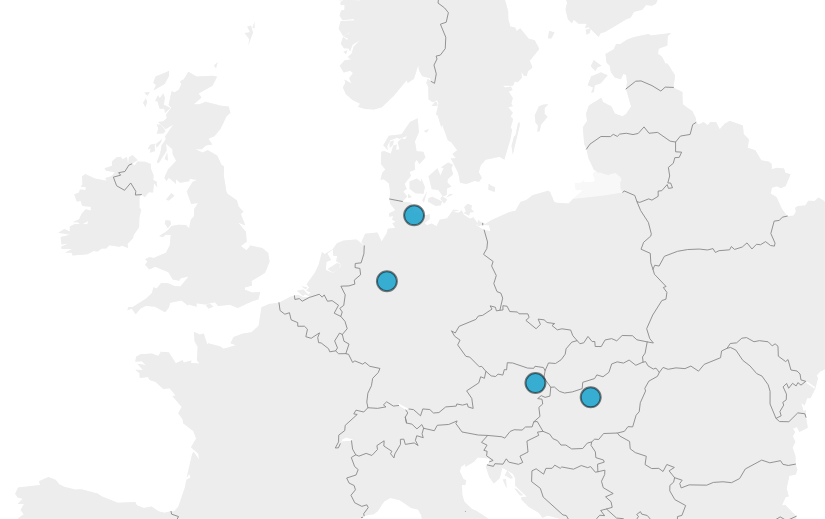
\includegraphics{images/authors-space.png}
\end{frame}

\section{Introduction}\label{introduction}

\begin{frame}{Research questions}
\protect\hypertarget{research-questions}{}
\begin{itemize}
\tightlist
\item
  How and where is open source software developed?
\item
  Can spatially dispersed developers produce quality software?
\item
  How do frictions affect collaboration and software quality?
\end{itemize}
\end{frame}

\begin{frame}{Two economic puzzles in open source}
\protect\hypertarget{two-economic-puzzles-in-open-source}{}
\begin{block}{Why do people work for free?}
\protect\hypertarget{why-do-people-work-for-free}{}
Altruism, reputation concerns, alternative business models. Sizeable
economic literature.
\end{block}

\begin{block}{How can spatially dispersed developers produce quality
software?}
\protect\hypertarget{how-can-spatially-dispersed-developers-produce-quality-software}{}
\end{block}
\end{frame}

\section{GitHub poll}\label{github-poll}

\section{\texorpdfstring{\texttt{if\ (poll\ ==\ "no")\ \{}}{if (poll == "no") \{}}\label{if-poll-no}

\begin{frame}{Why Open Source Software (OSS)?}
\protect\hypertarget{why-open-source-software-oss}{}
\begin{block}{OSS is huge}
\protect\hypertarget{oss-is-huge}{}
\begin{itemize}
\tightlist
\item
  Software industry -- 1\% of global GDP
\item
  90+\% of software has open source components
\end{itemize}
\end{block}

\begin{block}{OSS is everywhere}
\protect\hypertarget{oss-is-everywhere}{}
OSS plays an important roles in - Websites (PHP, JavaScript) - Operating
systems (Linux, Android) - Data (R Tidyverse, Python Pandas, Julia) -
Machine Learning and AI (PyTorch, LLaMA)
\end{block}

\begin{block}{OSS is observable}
\protect\hypertarget{oss-is-observable}{}
\end{block}
\end{frame}

\begin{frame}{A platform for sharing and discussing code}
\protect\hypertarget{a-platform-for-sharing-and-discussing-code}{}
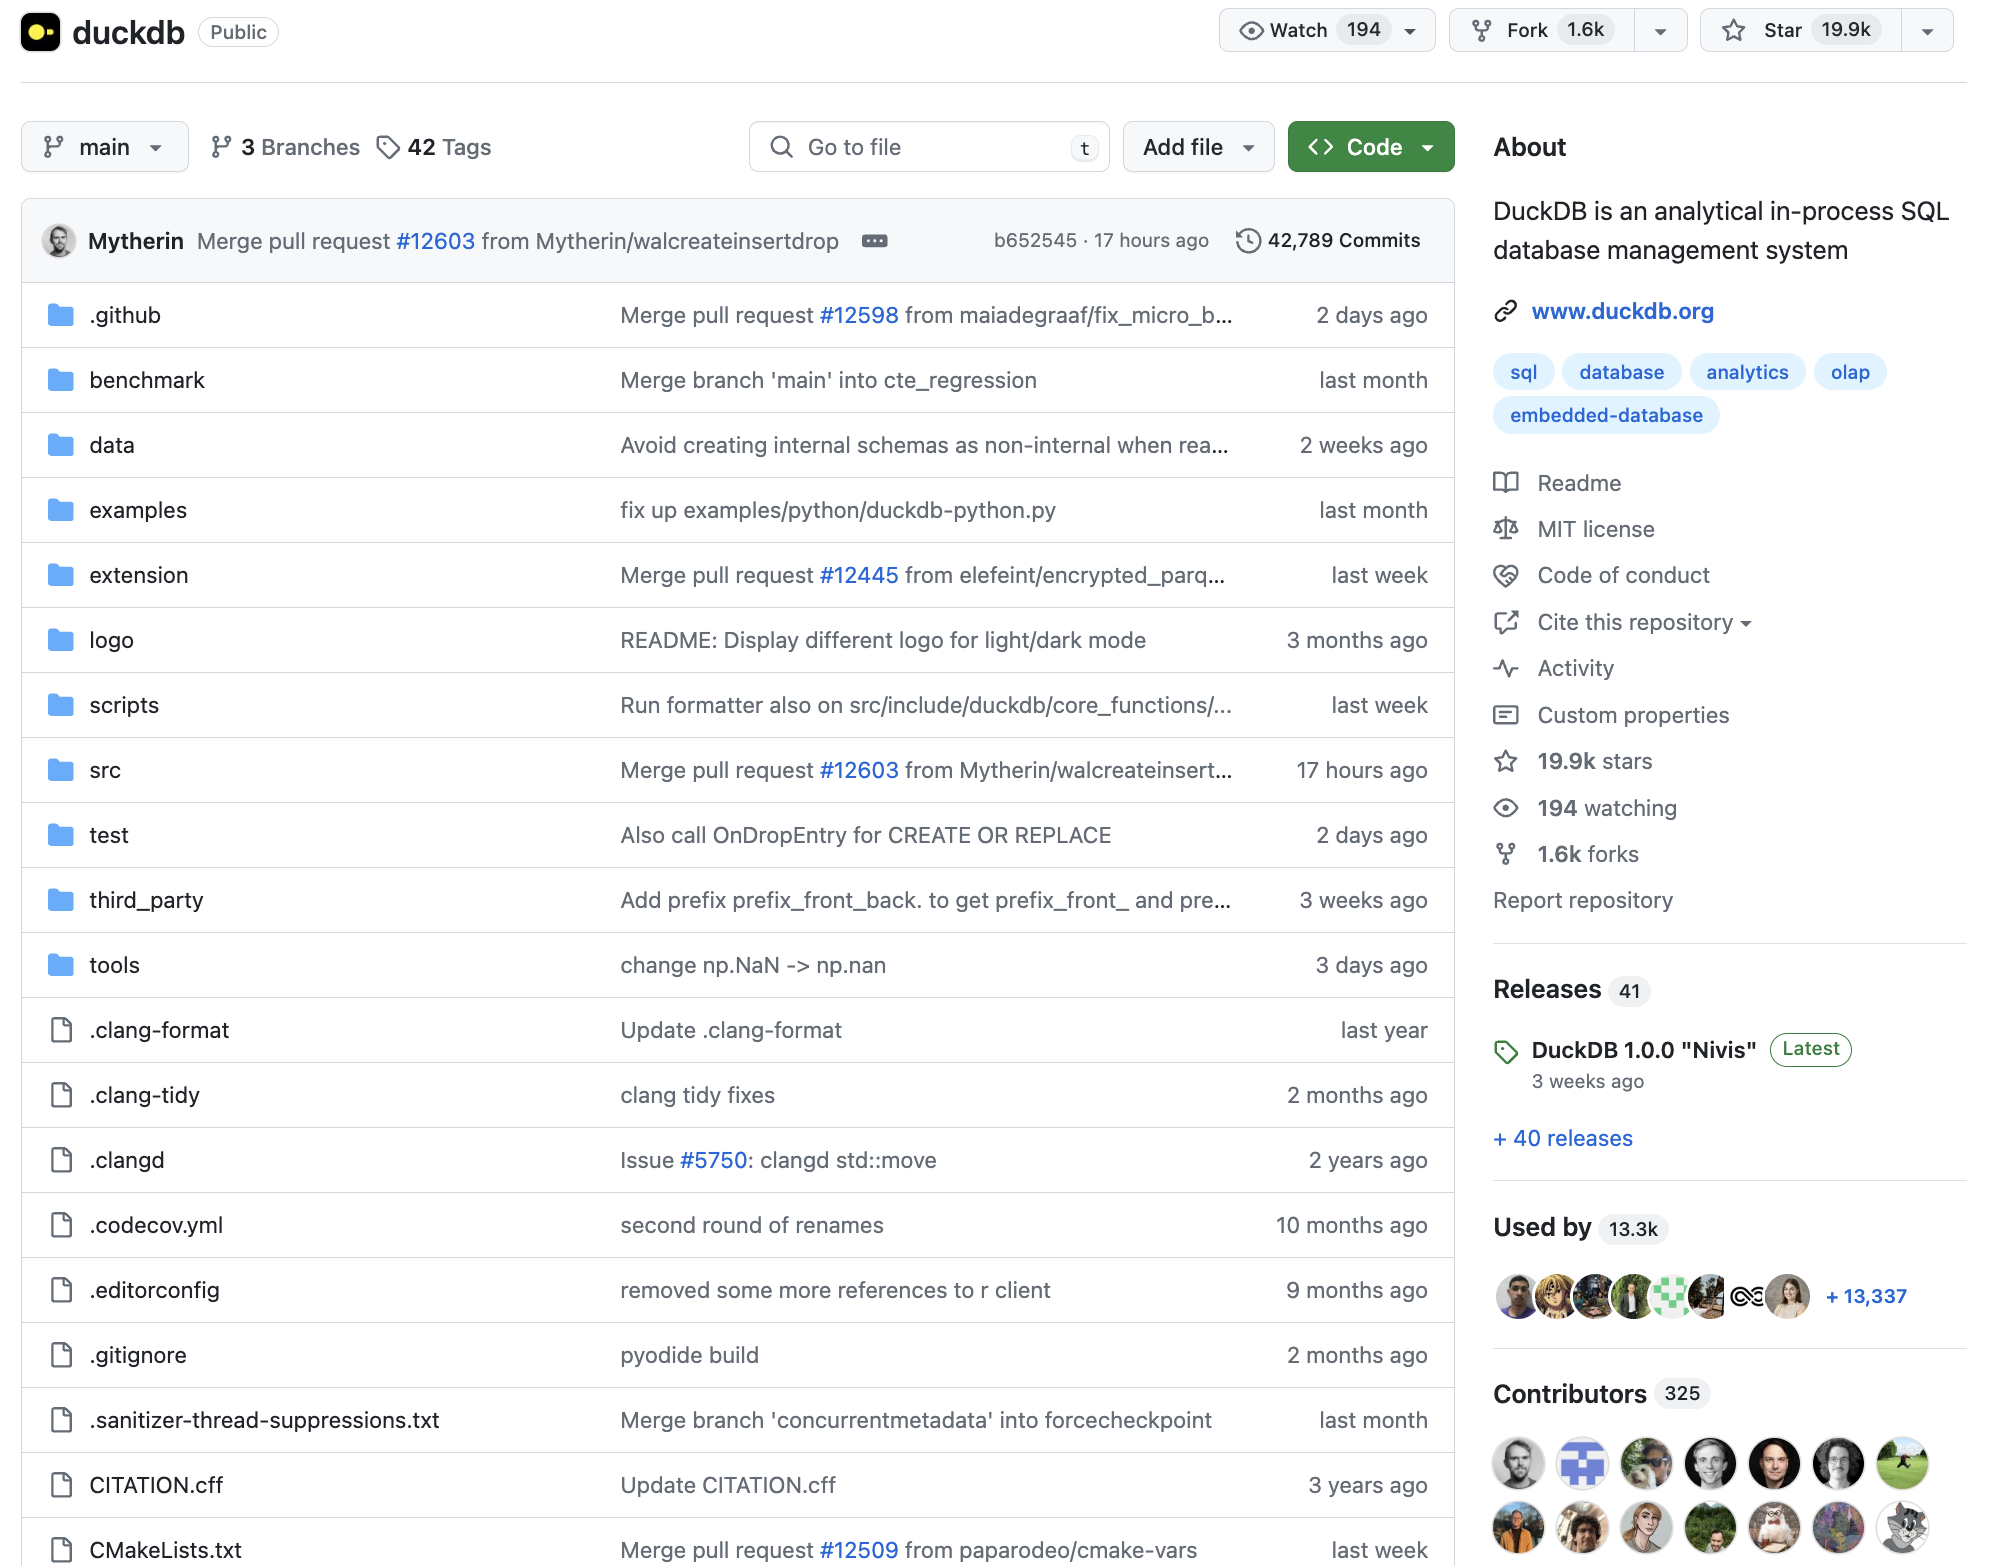
\includegraphics{images/duckdb-github.png}
\end{frame}

\begin{frame}{Not all developers contribute equally}
\protect\hypertarget{not-all-developers-contribute-equally}{}
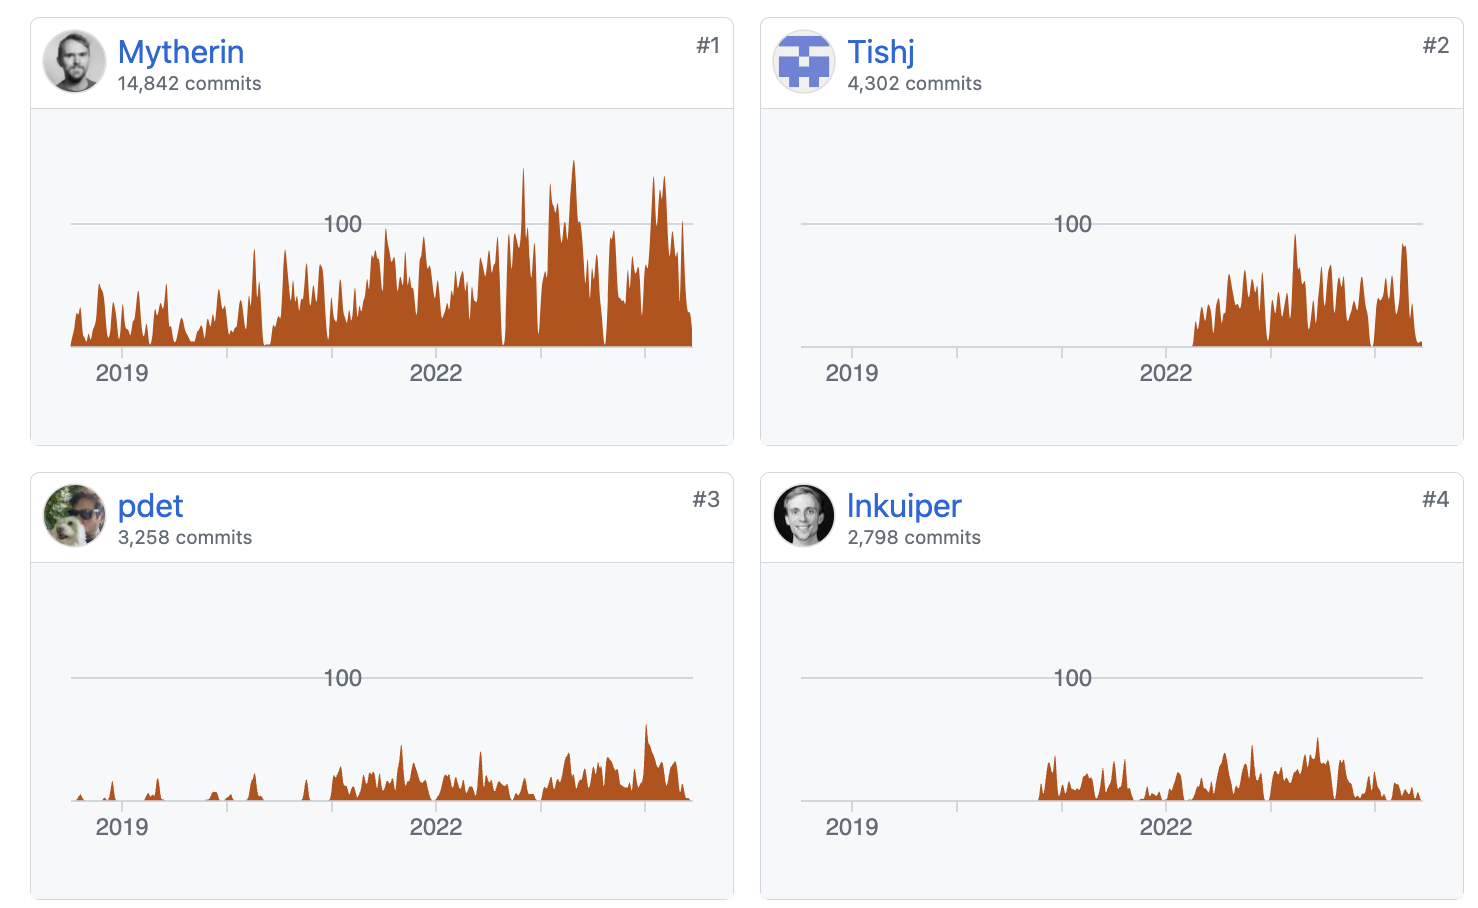
\includegraphics{images/collaboration-time.png}
\end{frame}

\begin{frame}{(Many) developers report their location}
\protect\hypertarget{many-developers-report-their-location}{}

\includegraphics{images/mike-waugh-github.png}
\end{frame}

\begin{frame}[fragile]{Open Source vocabulary}
\protect\hypertarget{open-source-vocabulary}{}
\texttt{Project}: A software project offering solution to a use case,
a.k.a. library, package.

\texttt{Repository}: A storage for one project (what we observe)

\texttt{Commit}: The smallest unit of contribution

\texttt{Git}: Distributed version control system for software projects

\texttt{GitHub}: A platform to collaboratively work on software projects

\texttt{Dependency}: An imported project that provides a functionality
\end{frame}

\section{\texorpdfstring{\texttt{\}}}{\}}}\label{section}

\begin{frame}{Related literature}
\protect\hypertarget{related-literature}{}
\begin{itemize}
\tightlist
\item
  \textbf{Geographical Distance / Network formation / Agglomeration}:
  {[}@chaney2014network{]} {[}@bernard2019production{]}
  {[}@davis2019spatial{]} {[}@BaileyGuptaHillenbrandEtAl2021{]},
  {[}@Atkin\_2022\_F2F{]}
\item
  \textbf{Gravity:} \textbf{Digital:} {[}@blum2006does{]}
  {[}@anderson2018dark{]}
\item
  \textbf{Frictions in services:} {[}@stein2007longitude{]}
  {[}@bahar2020hardships{]}
\item
  \textbf{Patents and science}: {[}@BircanJavorcikPauly2021{]},
  {[}@head\_li\_minondo\_math\_2019{]}, {[}@jaffe1993geographic{]},
  Singh (2008) {[}@AlShebli\_nature\_2018{]}, {[}@Li2014-patents-eer{]}
\item
  \textbf{OSS}: {[}@lerner2002some{]} , {[}@Laurentsyeva:2019{]}
  {[}@Wachs\_etal\_2022{]} {[}@fackler\_hofmann\_laurentsyeva\_2023{]}
\end{itemize}
\end{frame}

\begin{frame}{Outline}
\protect\hypertarget{outline}{}
\begin{enumerate}
\tightlist
\item
  Data and stylized facts about OSS production
\item
  A model of global team formation and collaboration
\item
  Test(able) implications
\end{enumerate}
\end{frame}

\section{Stylized facts}\label{stylized-facts}

\begin{frame}{Data}
\protect\hypertarget{data}{}
\begin{block}{GitHub}
\protect\hypertarget{github}{}
Snapshot of all public repositories on GitHub on 2019-06-01. Six largest
languages: JavaScript, Python, Java, Ruby, PHP, and C++. Drop smallest
and largest projects. 4.4m projects, 2.7m users. Self-reported location
for about 1/3 os users.
\end{block}

\begin{block}{libraries.io}
\protect\hypertarget{libraries.io}{}
Dependency data for projects on major package managers (npm, PyPI,
Maven, RubyGems, etc).
\end{block}
\end{frame}

\begin{frame}{JavaScript developer density around the globe}
\protect\hypertarget{javascript-developer-density-around-the-globe}{}
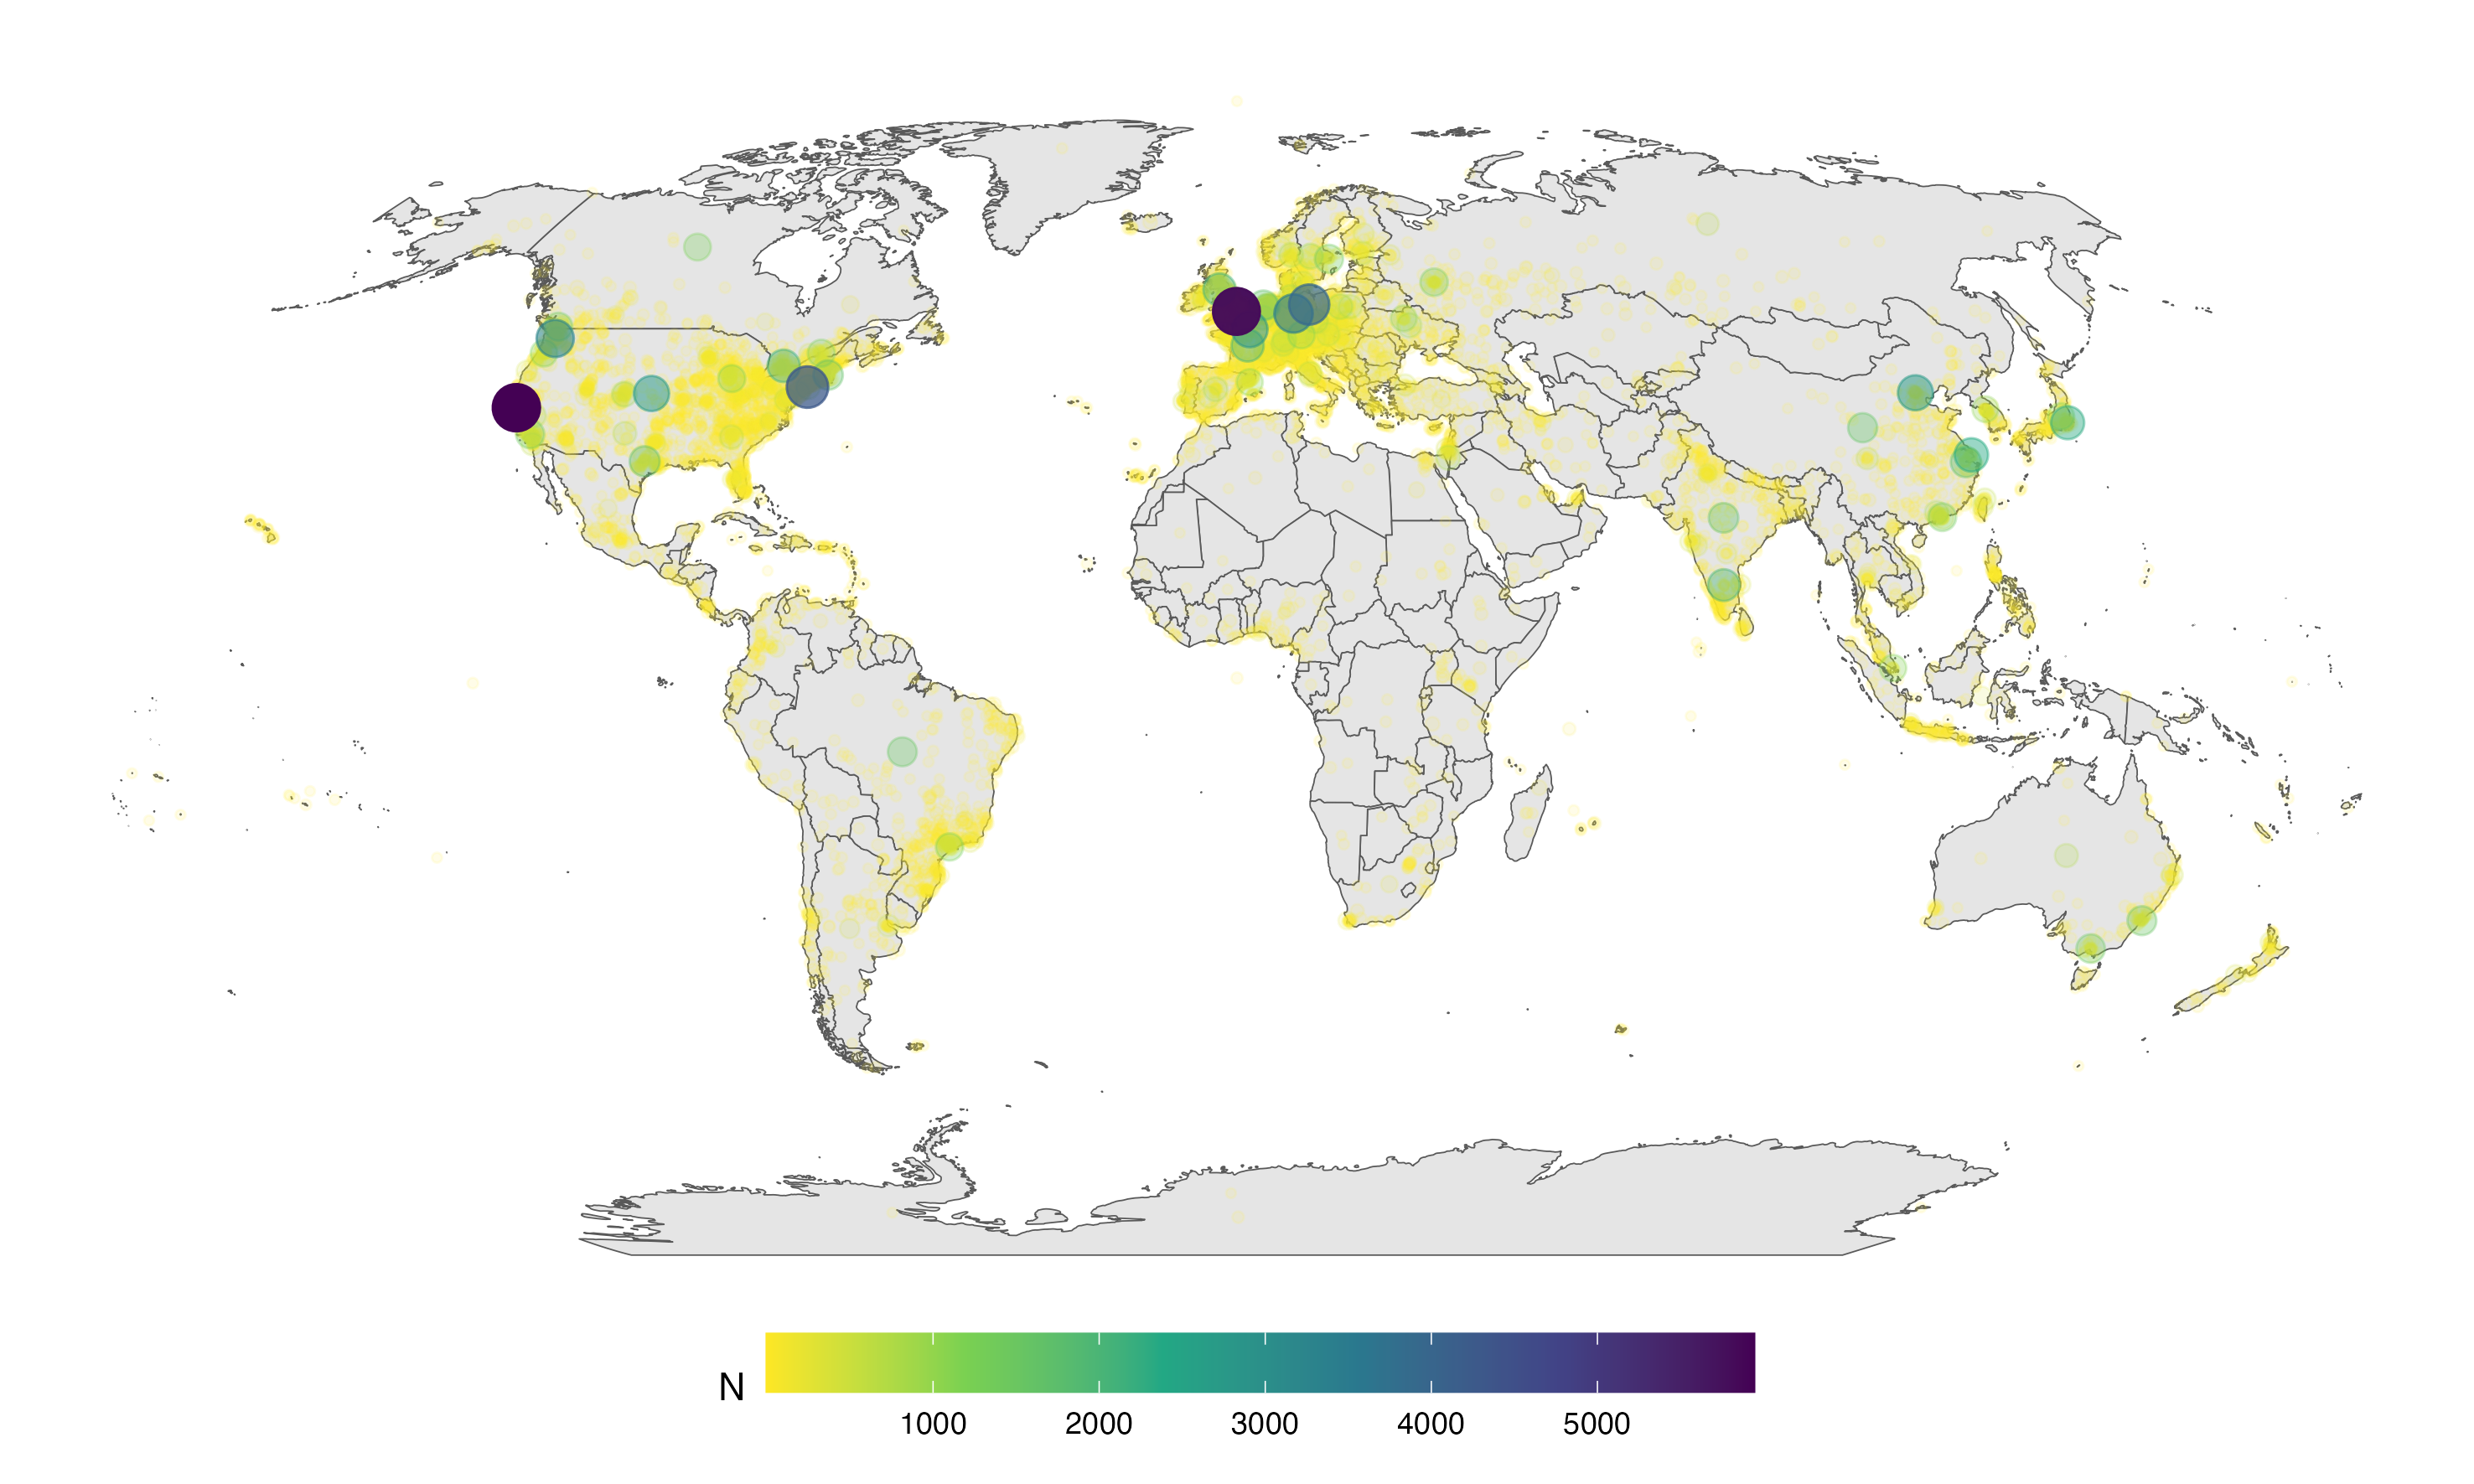
\includegraphics{figures/map_developers.png}
\end{frame}

\begin{frame}{Project size and popularity}
\protect\hypertarget{project-size-and-popularity}{}
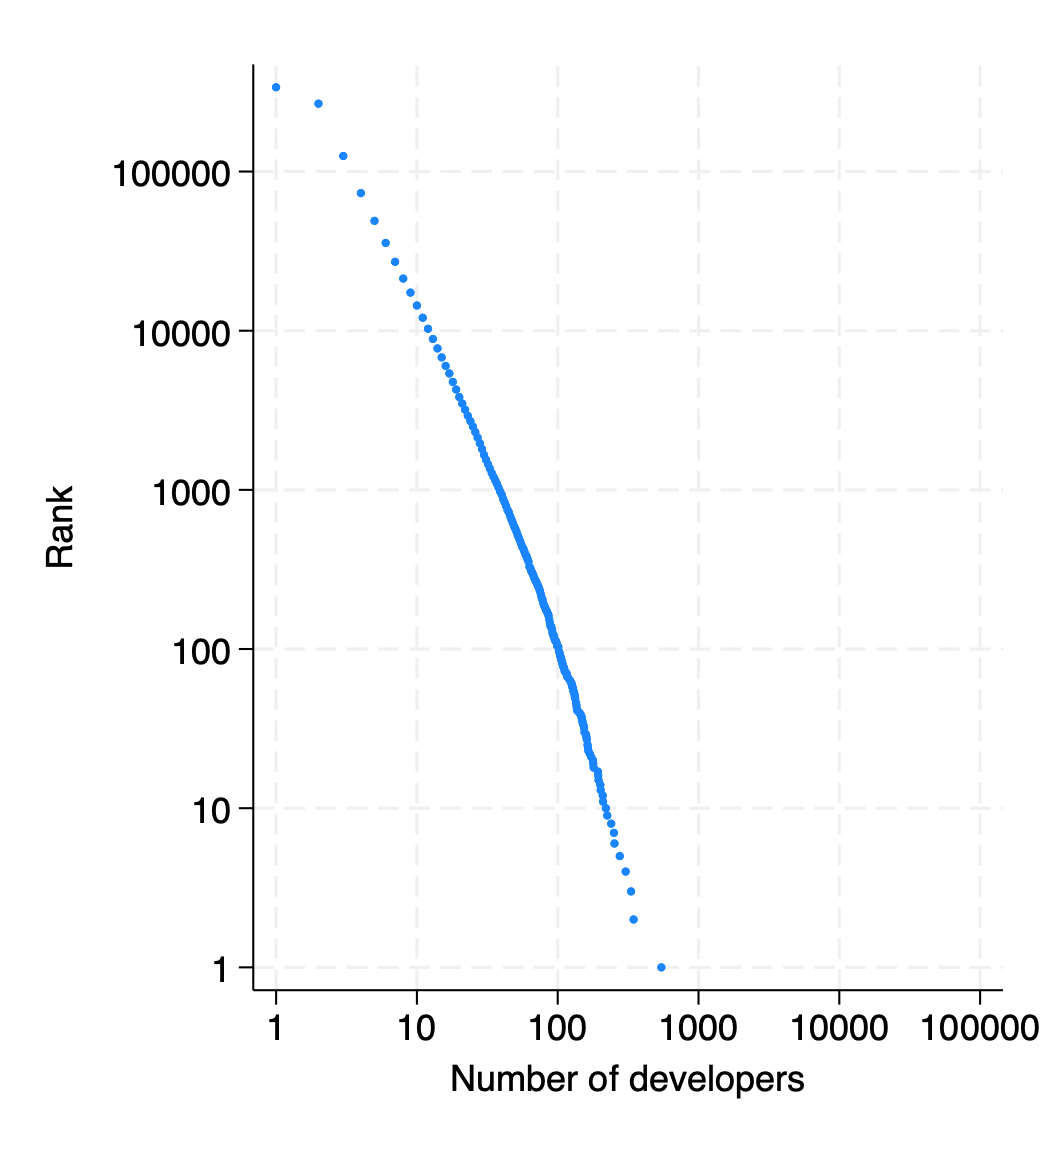
\includegraphics[width=0.45\textwidth,height=\textheight]{figures/developers_rank.png}
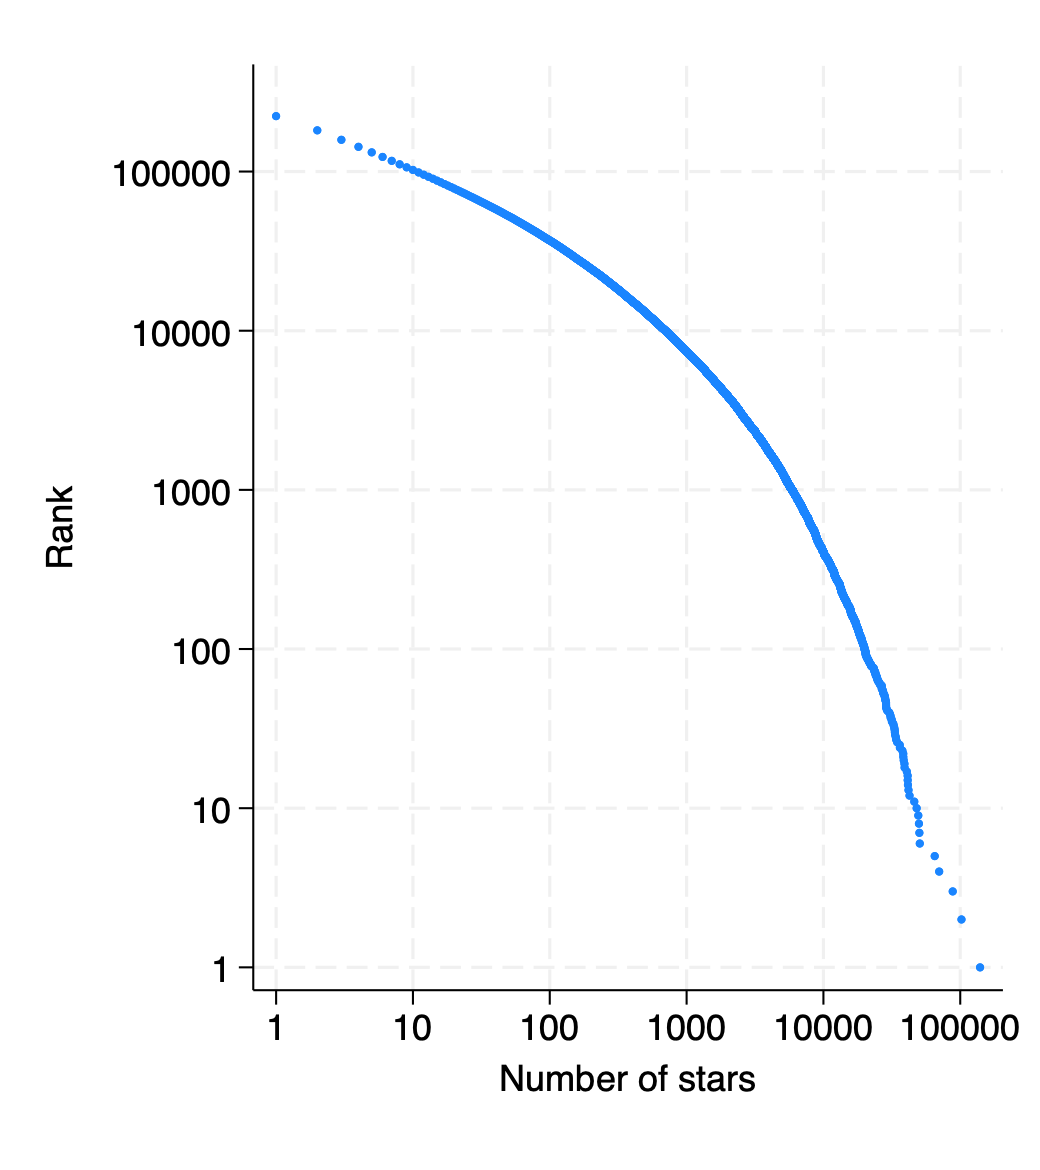
\includegraphics[width=0.45\textwidth,height=\textheight]{figures/stars_rank.png}
\end{frame}

\begin{frame}{Closer developers are more likely to contribute to the
same project}
\protect\hypertarget{closer-developers-are-more-likely-to-contribute-to-the-same-project}{}
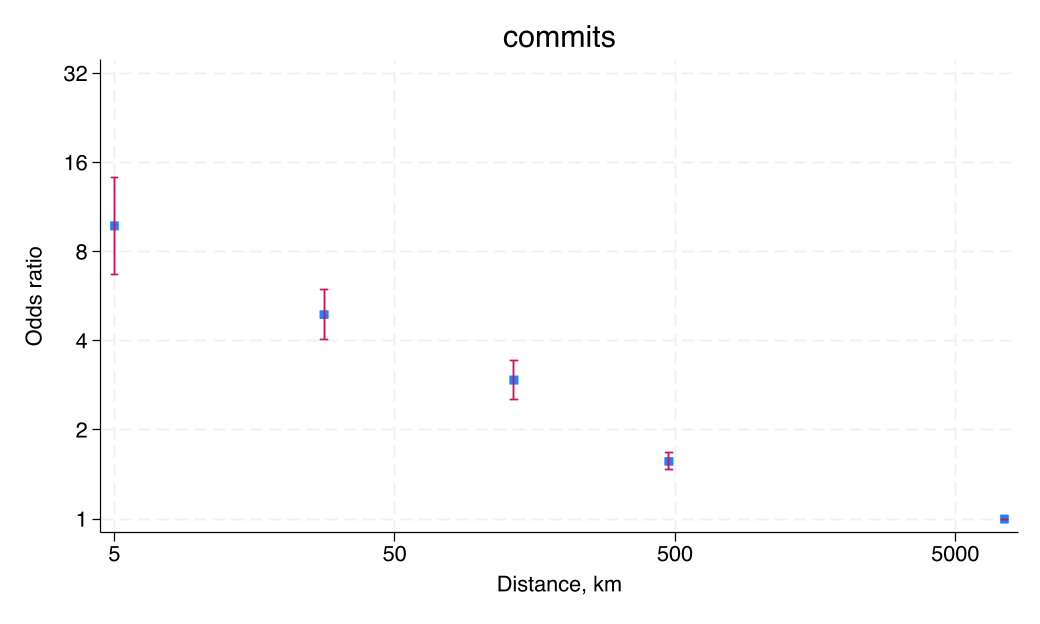
\includegraphics{figures/commits_gravity.png}
\end{frame}

\begin{frame}{There is no distance penalty for \emph{using} other's
software}
\protect\hypertarget{there-is-no-distance-penalty-for-using-others-software}{}
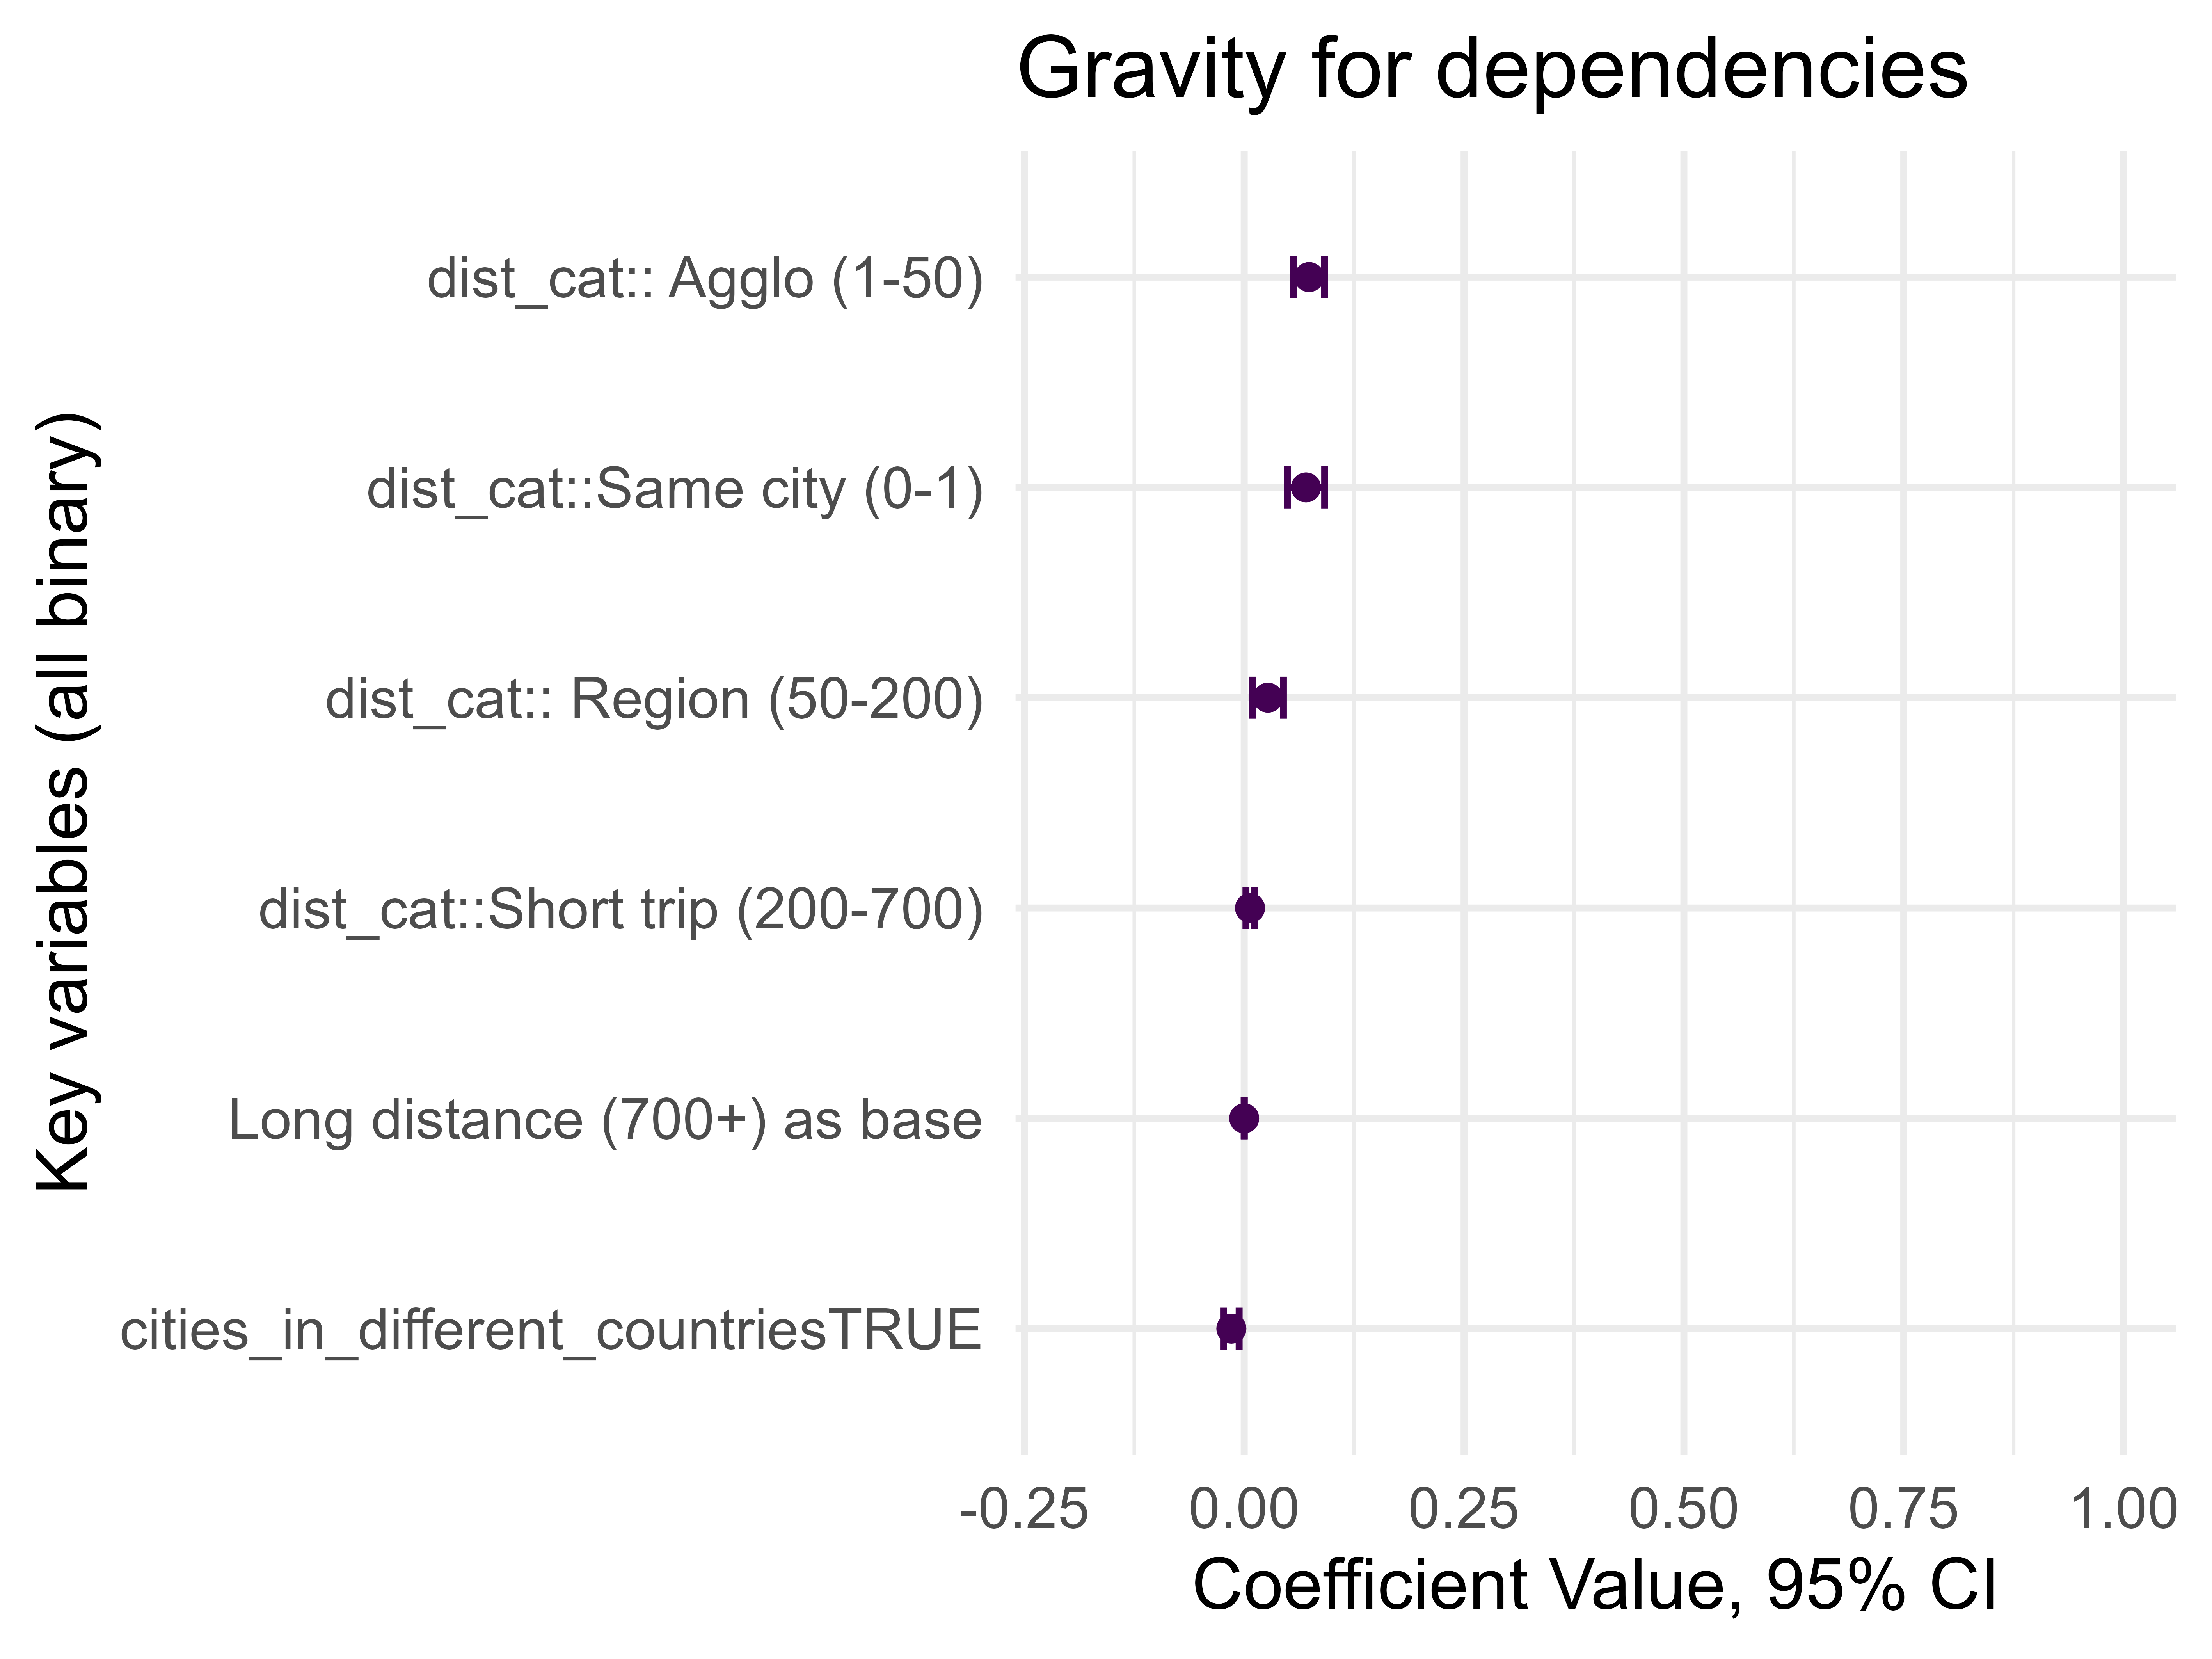
\includegraphics{figures/gravity_dependencies2.png}
\end{frame}

\begin{frame}{Better developers build more popular software, but
developers' skills are substitutes}
\protect\hypertarget{better-developers-build-more-popular-software-but-developers-skills-are-substitutes}{}
\vspace*{-2ex}\hspace*{-2em}
\begingroup
\centering
\begin{tabular}{lcccc}
   \tabularnewline \midrule \midrule
   Dependent Variable: & \multicolumn{4}{c}{n\_stars}\\
   Model:                                          & (1)            & (2)            & (3)            & (4)\\  
   \midrule
   \emph{Variables}\\
   log(stars\_lead)                                & 0.4707$^{***}$ &                & 0.4446$^{***}$ & 0.5086$^{***}$\\   
                                                   & (0.0260)       &                & (0.0535)       & (0.0618)\\   
   log(stars\_follow)                              &                & 0.2746$^{***}$ & 0.1600$^{***}$ & 0.2533$^{***}$\\   
                                                   &                & (0.0447)       & (0.0207)       & (0.0410)\\   
   log(stars\_lead) $\times$ log(stars\_follow)    &                &                &                & -0.0192$^{***}$\\   
                                                   &                &                &                & (0.0073)\\   
   \midrule
   \emph{Fixed-effects}\\
   lc                                              & Yes            & Yes            & Yes            & Yes\\  
   \midrule
   \emph{Fit statistics}\\
   Observations                                    & 17,906         & 17,339         & 3,348          & 3,348\\  
   Squared Correlation                             & 0.04906        & 0.01615        & 0.14126        & 0.13998\\  
   Pseudo R$^2$                                    & 0.22550        & 0.08336        & 0.29024        & 0.29179\\  
   BIC                                             & 3,426,757.9    & 2,498,745.2    & 628,673.9      & 627,311.3\\  
   \midrule \midrule
   \multicolumn{5}{l}{\emph{Clustered (lc) standard-errors in parentheses}}\\
   \multicolumn{5}{l}{\emph{Signif. Codes: ***: 0.01, **: 0.05, *: 0.1}}\\
\end{tabular}
\par\endgroup



\end{frame}

\section{Model}\label{model}

\begin{frame}{Model questions}
\protect\hypertarget{model-questions}{}
We take OSS payoffs as given.

higher software quality \(\to\) more payoff (``kudos'')

\begin{enumerate}
\tightlist
\item
  How do teams form?
\item
  How do they collaborate?
\item
  How do they distribute kudos?
\end{enumerate}
\end{frame}

\begin{frame}{Primitives}
\protect\hypertarget{primitives}{}
\begin{itemize}
\tightlist
\item
  Software developers vary in location, skill \(Z_i\) and preference for
  fame \(\xi_i\).
\item
  Fixed supply of developers at each location.
\item
  Team formation as well as collaboration across locations are costly.
\end{itemize}
\end{frame}

\begin{frame}{Timing}
\protect\hypertarget{timing}{}
\begin{enumerate}
\tightlist
\item
  Two developers meet at random

  \begin{itemize}
  \tightlist
  \item
    partially observe each other's skills
  \end{itemize}
\item
  Decide whether to do a project together

  \begin{itemize}
  \tightlist
  \item
    If not, enjoy outside option.
  \end{itemize}
\item
  Software is developed to a certain quality.
\item
  Users download it, distributing kudos to developers.
\end{enumerate}
\end{frame}

\begin{frame}{Model outline}
\protect\hypertarget{model-outline}{}
\begin{tikzpicture}
    % Nodes
    \node[draw, rectangle] (O1) at (2, 1) {opportunity cost 1};
    \node[draw, rectangle] (J1) at (2, 3) {payoff 1};
    \node[draw, rectangle] (J2) at (2, -3) {payoff 2};
    \node[draw, rectangle] (O2) at (2, -1) {opportunity cost 2};
    \node[draw, rectangle] (T1) at (4, 2) {developer skill 1};
    \node[draw, rectangle] (T2) at (4, -2) {developer skill 2};
    \node[draw, rectangle] (F) at (6, 0) {software quality};
    \node[draw, rectangle] (K) at (10, 0) {kudos};
    
    % Edges
    \draw[->] (O1) -- (T1);
    \draw[->] (J1) -- (T1);
    \draw[->] (O2) -- (T2);
    \draw[->] (J2) -- (T2);
    \draw[->, bend right] (K) to (J1);
    \draw[->, bend left] (K) to (J2);
    \draw[->] (F) -- (K);
    \draw[->] (T1) -- (F);
    \draw[->] (T2) -- (F);
\end{tikzpicture}
\end{frame}

\begin{frame}{Spatial frictions}
\protect\hypertarget{spatial-frictions}{}
\begin{tikzpicture}
    % Nodes
    \node[draw, rectangle] (O1) at (2, 1) {opportunity cost 1};
    \node[draw, rectangle] (J1) at (2, 3) {payoff 1};
    \node[draw, rectangle] (J2) at (2, -3) {payoff 2};
    \node[draw, rectangle] (O2) at (2, -1) {opportunity cost 2};
    \node[draw, rectangle] (T1) at (4, 2) {developer skill 1};
    \node[draw, rectangle] (T2) at (4, -2) {developer skill 2};
    \node[draw, rectangle] (F) at (6, 0) {software quality};
    \node[draw, rectangle] (K) at (10, 0) {kudos};
    
    % Edges
    \draw[->] (O1) -- (T1);
    \draw[->] (J1) -- (T1);
    \draw[->] (O2) -- (T2);
    \draw[->] (J2) -- (T2);
    \draw[->, bend right, blue, line width=1mm] (K) to (J1);
    \draw[->, bend left, blue, line width=1mm] (K) to (J2);
    \draw[->] (F) -- (K);
    \draw[->, red, line width=1mm] (T1) -- (F);
    \draw[->, red, line width=1mm] (T2) -- (F);
\end{tikzpicture}
\end{frame}

\begin{frame}{Team composition}
\protect\hypertarget{team-composition}{}
Project \(p\) is developed by two developers with skills \(Z_1\) and
\(Z_2\).

Developer skill drawn from Fréchet distribution: \[
\Pr(Z_i \le x) = e^{-T_{ip}x^{-\theta}}
\]

\begin{block}{Developer skill}
\protect\hypertarget{developer-skill}{}
\(T_{ip}\) observable (programming language, years of experience, etc.)

\(1/\theta\) captures importance of unobservable skill
\end{block}
\end{frame}

\begin{frame}{Software production function}
\protect\hypertarget{software-production-function}{}
Software quality depends on the best idea: \[
X_p := \max \{Z_{1p}, Z_{2p}/\tau_{2p}\}
\]

\begin{block}{Knowledge sharing cost}
\protect\hypertarget{knowledge-sharing-cost}{}
\(\tau_{ip} \ge 1\). Not all good ideas are heard (language, time zone,
culture, clarity).

Normalize \(\tau_{1p}=1\) for presentation.
\end{block}

\begin{block}{Gravity}
\protect\hypertarget{gravity}{}
\[
\tau_{ip} = \text{distance}_{ip}^{\gamma_k}
\]
\end{block}
\end{frame}

\begin{frame}{Distribution of software quality}
\protect\hypertarget{distribution-of-software-quality}{}
Software quality is also Fréchet. \[
\Pr(X_p \le x) = e^{-\Phi_p x^{-\theta}}
\] with \[
\Phi_p := T_{1p} + \tau_{2p}^{-\theta}T_{2p}
\]

\begin{block}{Testable implications}
\protect\hypertarget{testable-implications}{}
\begin{enumerate}
\tightlist
\item
  Larger teams produce better software.
\item
  Better developers produce better software.
\item
  Knowledge sharing frictions reduce software quality.
\end{enumerate}
\end{block}
\end{frame}

\begin{frame}{Sharing kudos}
\protect\hypertarget{sharing-kudos}{}
Overall customer happiness increases in software quality: \[
V_p := e^{X_p}
\]

\begin{block}{Attribution of kudos}
\protect\hypertarget{attribution-of-kudos}{}
The better-skilled developer gets all the kudos for \(V_p\).
(\(\approx\) ``First author bias'')
\end{block}
\end{frame}

\begin{frame}{Expected developer payoff from project \(p\)}
\protect\hypertarget{expected-developer-payoff-from-project-p}{}
\[
\mathcal U_{ip} = \begin{cases}
e^{\xi_i Z_i/\tau_{ip}} & \text{if }Z_i/\tau_{ip} > Z_j/\tau_{jp}\\
0 & \text{otherwise}
\end{cases}
\] where \(\xi_i\) is a taste parameter for enjoying kudos. In
expectation, \[
U_{ip} = \text{E}\,\mathcal U_{ip} =
e^{-T_{jp}\tau_{ip}^\theta Z_i^{-\theta}}
e^{\xi Z_i/\tau_{ip}}
\] Increases in \(Z_i\), decreases in \(T_{jp}\), \(\tau_{ip}\).
\end{frame}

\begin{frame}{Team formation}
\protect\hypertarget{team-formation}{}
Does developer \(i\) join project \(p\)? \[
U_{ip}(Z_i, T_{jp}, \xi_i) > \text{cost}_{i}(Z_i, d_{ip}) := e^{d_{ip}\xi_i Z_i}
\]

\begin{block}{Distribution cost}
\protect\hypertarget{distribution-cost}{}
\(d_{ip} \ge 1\). Not all benefits of distant projects can be captured
(private cost of participation, time zones, misappropriate of credit).
\end{block}

\begin{block}{Gravity}
\protect\hypertarget{gravity-1}{}
\[
d_{ip} = \text{distance}_{ip}^{\gamma_s} 
\] where \(\gamma_s\) may be different from \(\gamma_k\)
\end{block}
\end{frame}

\begin{frame}{Join team \(p\) if}
\protect\hypertarget{join-team-p-if}{}
\[
Z_i > \frac{\tau_{ip} T_{jp}^{1/(\theta+1)} }
{(\tau_{ip} d_{ip} - 1)^{1/(\theta+1)}} 
\xi_i^{-1/(\theta+1)}
\]

\begin{block}{Selection}
\protect\hypertarget{selection}{}
\begin{enumerate}
\tightlist
\item
  Better skilled developers are more likely to join.
\item
  Spatial frictions reduce team formation.
\item
  Projects with high-skilled developers are more selective.
\end{enumerate}
\end{block}
\end{frame}

\begin{frame}{Fréchet magic}
\protect\hypertarget{fruxe9chet-magic}{}
Assume \(Z_i\) is Fréchet with parameters \(T_i\) and \(\theta\),

\(\xi_i\) is Weibull with \(\kappa\) and \(\theta/(\theta+1)\). Then \[
\Pr(Z_i \le x | i\text{ joins project }p) = e^{-T_{ip}x^{-\theta}}
\] with \[
T_{ip} = T_i + \frac1\kappa \frac{\tau_{ip}^\theta T_{jp}^{\theta/(\theta+1)} }
{(\tau_{ip} d_{ip} - 1)^{\theta/(\theta+1)}}
\]
\end{frame}

\begin{frame}{Closing the model}
\protect\hypertarget{closing-the-model}{}
Both developers want to join, knowing what to expect from the other.

\begin{block}{Mutual coincidence of wants}
\protect\hypertarget{mutual-coincidence-of-wants}{}
\[
\begin{aligned}
T_{1p} & = T_1 + \frac1\kappa \frac{T_{2p}^{\theta/(\theta+1)} }
{(d_{1p} - 1)^{\theta/(\theta+1)}} \\
T_{2p} &= T_2 + \frac1\kappa \frac{\tau_{2p}^\theta T_{1p}^{\theta/(\theta+1)} }
{(\tau_{2p} d_{2p} - 1)^{\theta/(\theta+1)}}
\end{aligned}
\]
\end{block}

\begin{block}{Team forms with probability}
\protect\hypertarget{team-forms-with-probability}{}
\[
\frac{T_1}{T_{1p}}
\frac{T_2}{T_{2p}}
\]
\end{block}
\end{frame}

\section{Testable predictions}\label{testable-predictions}

\begin{frame}{Testable predictions}
\protect\hypertarget{testable-predictions-1}{}
\begin{block}{Gravity of team formation}
\protect\hypertarget{gravity-of-team-formation}{}
\begin{enumerate}
\tightlist
\item
  Distant developers are less likely to join a team.
\end{enumerate}
\end{block}

\begin{block}{Knowledge production}
\protect\hypertarget{knowledge-production}{}
\begin{enumerate}
\setcounter{enumi}{1}
\tightlist
\item
  Two-person projects are better than one-person projects.
\item
  Projects with better developers are more successful.
\item
  Project success depends disproportionately on ``lead developer.''
\end{enumerate}
\end{block}

\begin{block}{Assortative matching}
\protect\hypertarget{assortative-matching}{}
\begin{enumerate}
\setcounter{enumi}{4}
\tightlist
\item
  Skilled developers team up with skilled developers.
\end{enumerate}
\end{block}

\begin{block}{Selection}
\protect\hypertarget{selection-1}{}
\begin{enumerate}
\setcounter{enumi}{5}
\tightlist
\item
  Projects with distant developers are more successful.
\item
  But not if we condition on developer skill.
\end{enumerate}
\end{block}
\end{frame}

\section{Results}\label{results}

\begin{frame}{Measuring skill and quality}
\protect\hypertarget{measuring-skill-and-quality}{}
\begin{block}{Developer skill}
\protect\hypertarget{developer-skill-1}{}
\begin{enumerate}
\tightlist
\item
  Commits in other projects
\item
  Days worked on other projects
\item
  Total stars on other projects
\end{enumerate}
\end{block}

\begin{block}{Software quality}
\protect\hypertarget{software-quality}{}
\begin{enumerate}
\tightlist
\item
  Number of stars
\item
  Number of downstream libraries
\end{enumerate}
\end{block}
\end{frame}

\begin{frame}{Two-person projects have better developers}
\protect\hypertarget{two-person-projects-have-better-developers}{}
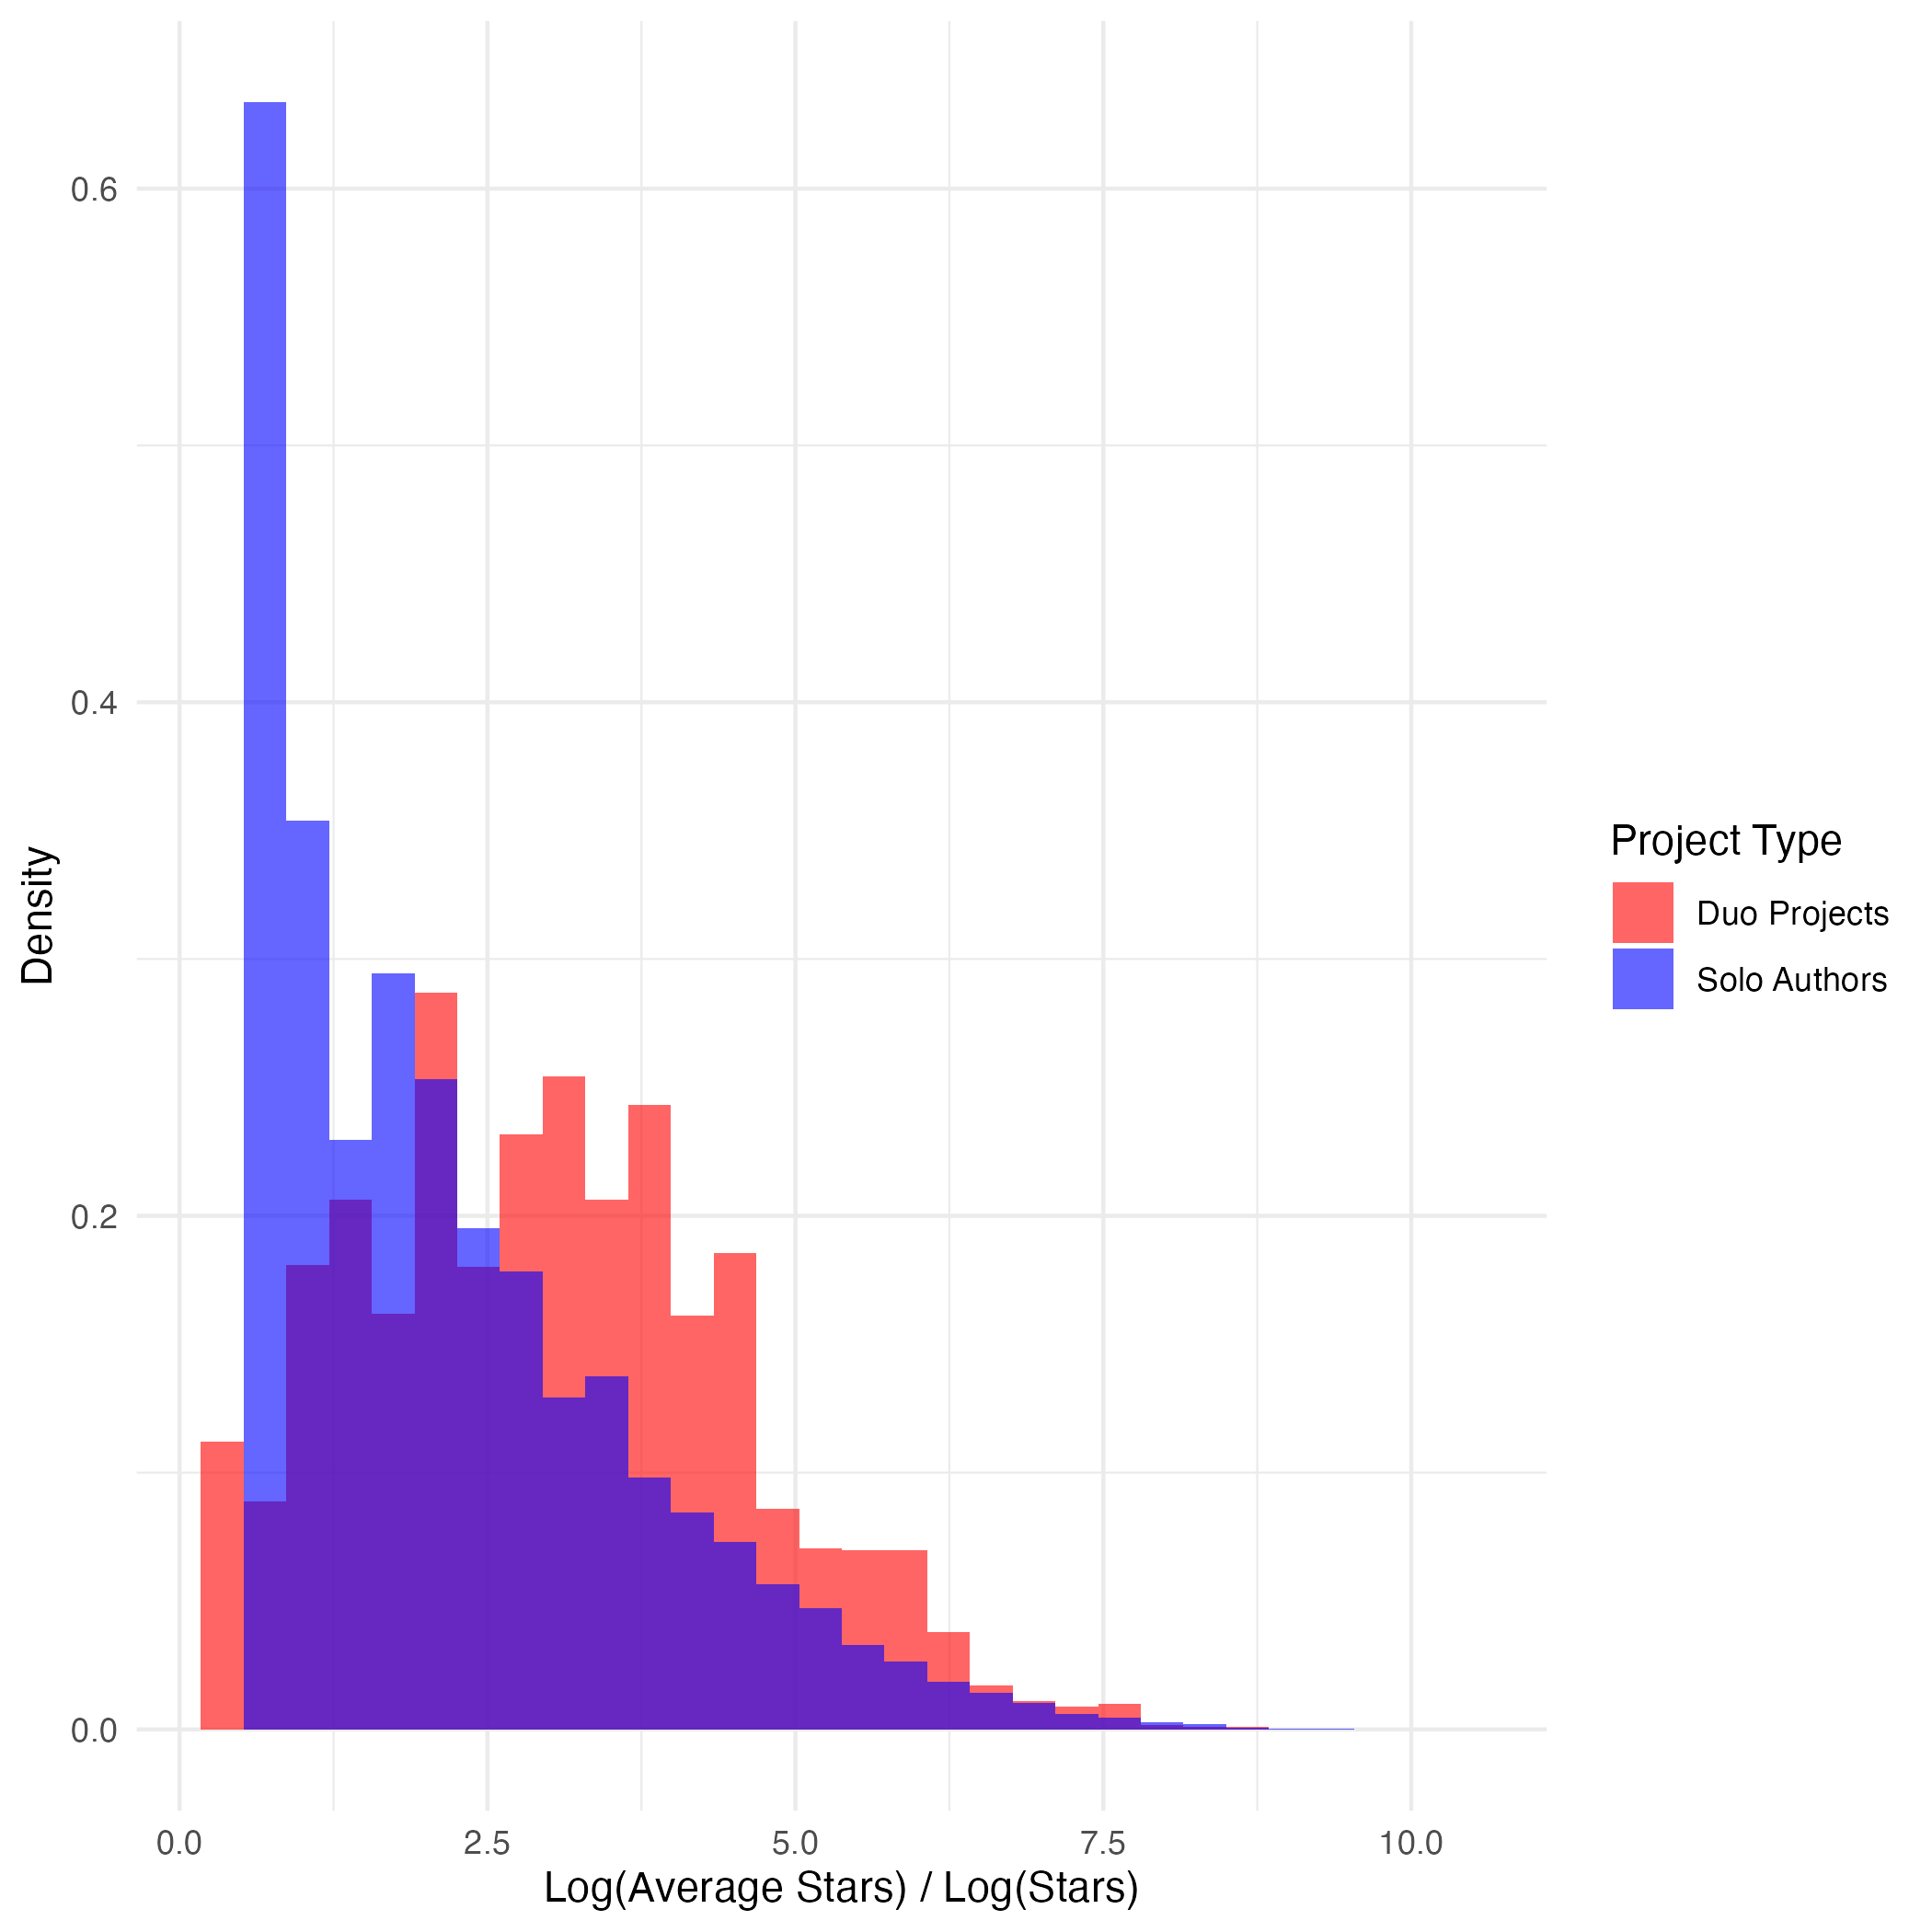
\includegraphics{figures/coder_quality_solo_duo.png}
\end{frame}

\begin{frame}{Leaders are better than followers}
\protect\hypertarget{leaders-are-better-than-followers}{}
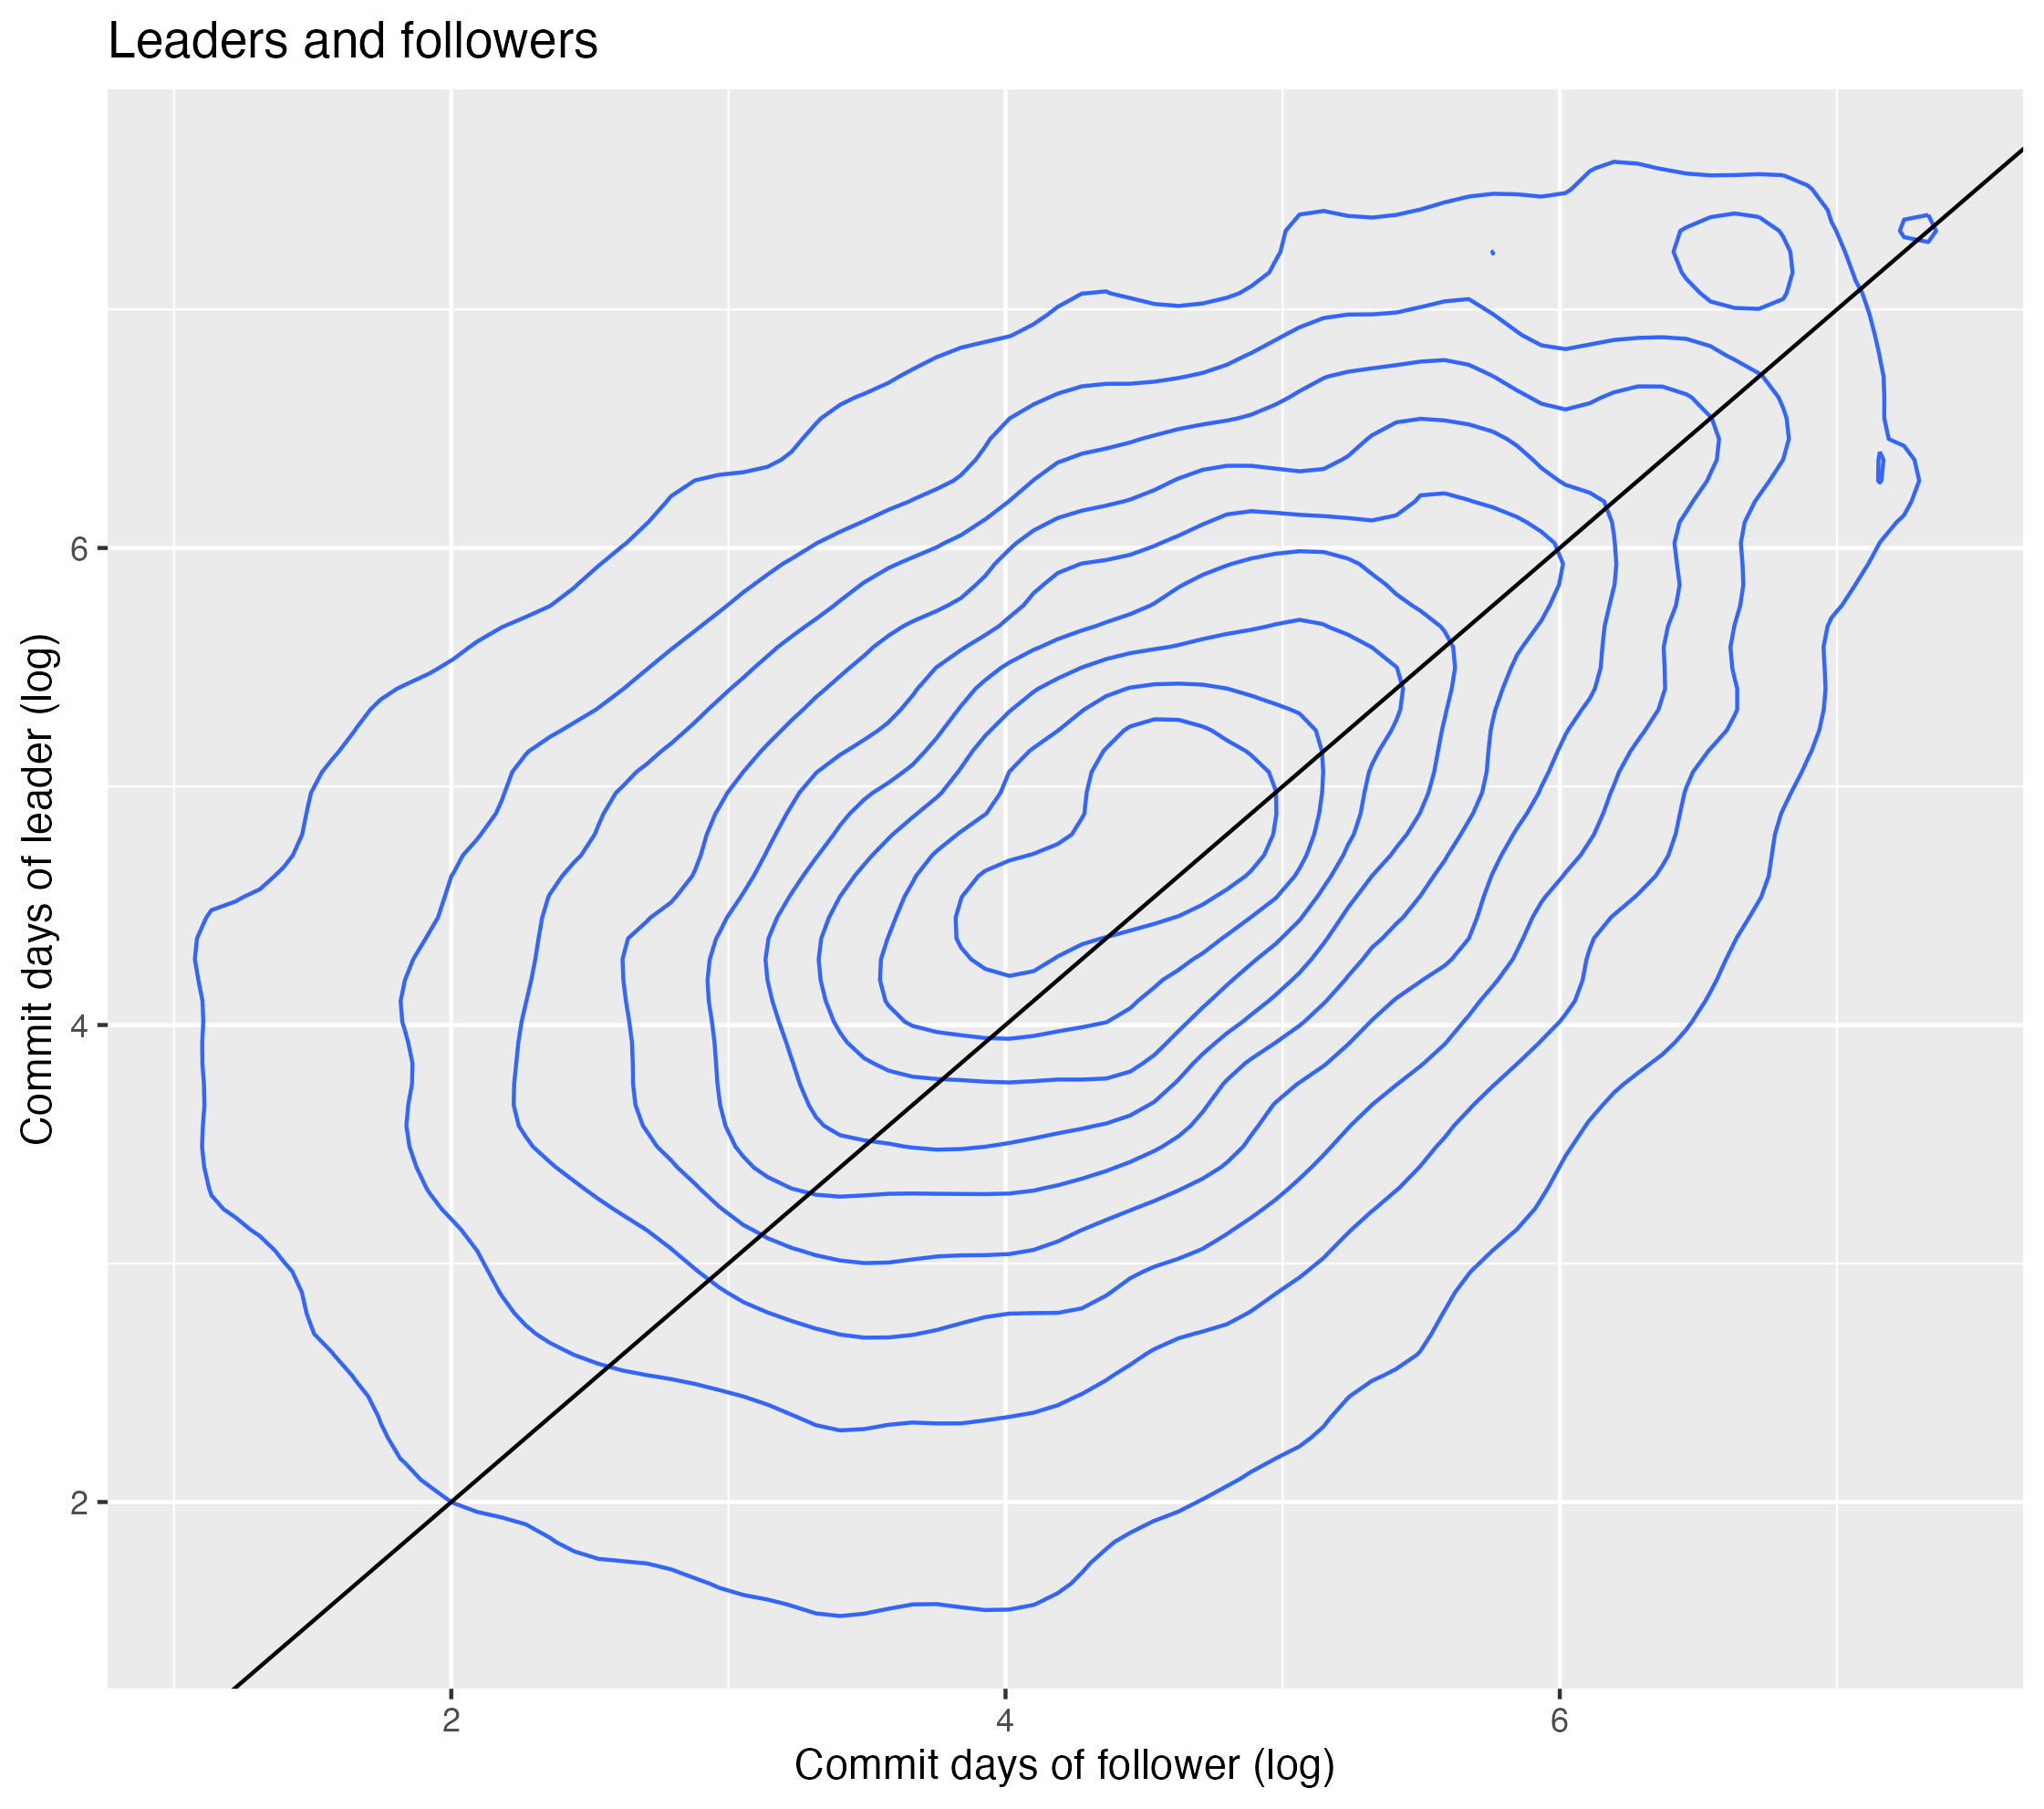
\includegraphics{figures/quality_scatter.png}
\end{frame}

\section{Collaboration in space}\label{collaboration-in-space}

\begin{frame}{Gravity model of collaboration}
\protect\hypertarget{gravity-model-of-collaboration}{}
Developer \(i\) and \(j\) collaborate with probability \[
\Pr(\text{Collaboration}_{ij}) = \exp(\alpha_i + \beta_j -\gamma\times\text{distance}_{ij})
\] Aggregate across city pairs \(d\) and \(o\): \[
E(N_{do,\text{collab}}) = N_o\times N_d\times\exp(\tilde\alpha_d + \tilde\beta_o -\gamma\times\text{distance}_{do})
\] Estimate this with Poisson maximum likelihood.
\end{frame}

\begin{frame}{Gravity of team formation across languages}
\protect\hypertarget{gravity-of-team-formation-across-languages}{}
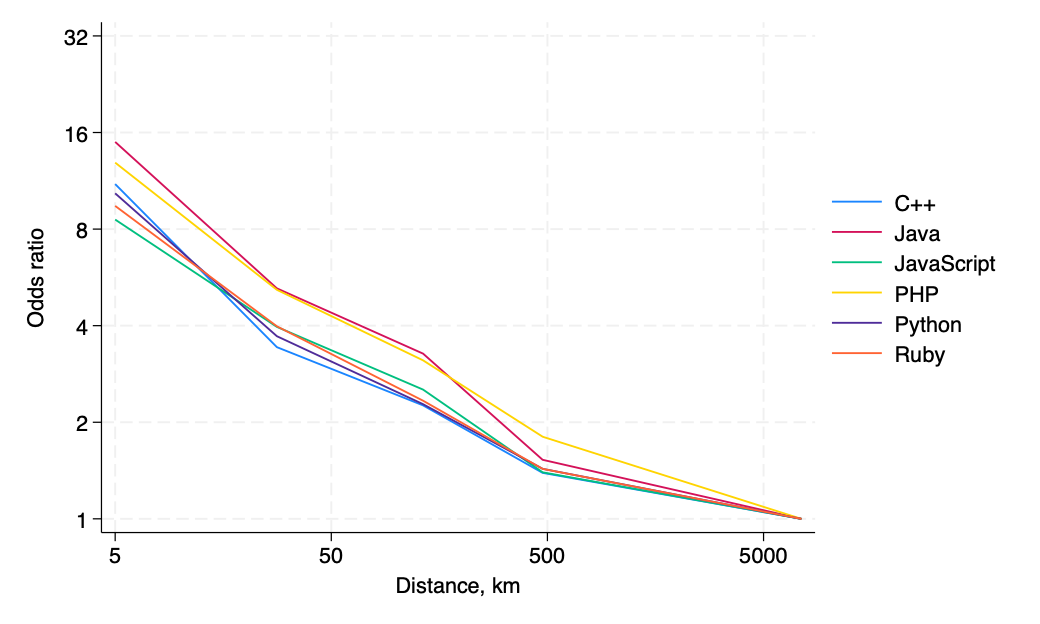
\includegraphics{figures/commits_by_language.png}
\end{frame}

\begin{frame}{Frictions reduce work but increase quality}
\protect\hypertarget{frictions-reduce-work-but-increase-quality}{}
\vspace*{-2ex}\hspace*{-2em}
\begingroup
\centering
\begin{tabular}{lcccc}
   \tabularnewline \midrule \midrule
   Dependent Variables: & n\_commits      & n\_days         & n\_stars       & n\_downstream\\   
   Model:               & (1)             & (2)             & (3)            & (4)\\  
   \midrule
   \emph{Variables}\\
   Average distance (km, log)    & 0.0399$^{***}$  & 0.0217$^{***}$  & 0.2252$^{***}$ & 0.3326$^{***}$\\   
                        & (0.0042)        & (0.0011)        & (0.0113)       & (0.0522)\\   
   No.~cities (log)        & -0.1557$^{***}$ & -0.1528$^{***}$ & 0.3228$^{***}$ & 1.830$^{***}$\\   
                        & (0.0303)        & (0.0072)        & (0.0805)       & (0.3505)\\   
   No.~countries (log)     & -0.2569$^{***}$ & -0.2199$^{***}$ & 0.4845$^{***}$ & 0.9514$^{***}$\\   
                        & (0.0233)        & (0.0047)        & (0.0473)       & (0.2028)\\   
   No.~developers (log)    & 1.235$^{***}$   & 1.100$^{***}$   & 0.5690$^{***}$ & -1.506$^{***}$\\   
                        & (0.0295)        & (0.0067)        & (0.0843)       & (0.3246)\\   
   \midrule
   \emph{Fit statistics}\\
   Observations         & 267,086         & 267,086         & 267,086        & 267,086\\  
   Pseudo R$^2$         & 0.24991         & 0.40519         & 0.42086        & 0.23597\\  
   \midrule \midrule
   \multicolumn{5}{l}{\emph{Clustered (project\_id) standard-errors in parentheses}}\\
   \multicolumn{5}{l}{\emph{Signif. Codes: ***: 0.01, **: 0.05, *: 0.1}}\\
\end{tabular}
\par\endgroup



\end{frame}

\section{Conclusion}\label{conclusion}

\begin{frame}{Conclusion}
\begin{enumerate}
\tightlist
\item
  Tractable modle of global team formation and collaboration.
\item
  Team formation in OSS is highly localized.
\item
  Spatial diversity is associated with higher quality of work.
\end{enumerate}
\end{frame}

\begin{frame}{Get in touch}
\protect\hypertarget{get-in-touch}{}
@GaborBekes, @JulianHinz, @korenmiklos
\end{frame}

\end{document}
